\documentclass[12pt]{article}
\usepackage[utf8]{inputenc}
\usepackage{graphicx}
\usepackage[a4paper,width=200mm,top=25mm,bottom=25mm]{geometry}

\title{
{
\includegraphics[width=12cm, height=10cm]{images/csedu_logo.png}}\\
{\large Department of Computer Science and Engineering,\\      University of Dhaka}\\
{ Lab Report for Lab 2 }
}



\author{ Submitted by: Prothito Shovon Majumder \\ Submitted to: Dr. Upama Kabir }



\begin{document}
\maketitle

\newpage
\section{Task 1}

\subsection{Detailed Explanation of the Code:}
The solution to this problem is similar to the sample problem. The solution process is as follows: 
\begin{itemize}
    \item Store the variables X, Y and Z in registers r4, r3 and r2 respectively.
    \item Store the sum of X and Y in register r1.
    \item Add Z to the previously computed sum to calculate W and store it in register r1.
    \item Equate the variables X, Y and Z to 9, 8 and 5 respectively.
\end{itemize}
\subsection{Screenshot of the System State after Loading the Code:}
\begin{figure}[ht]
    \centering
    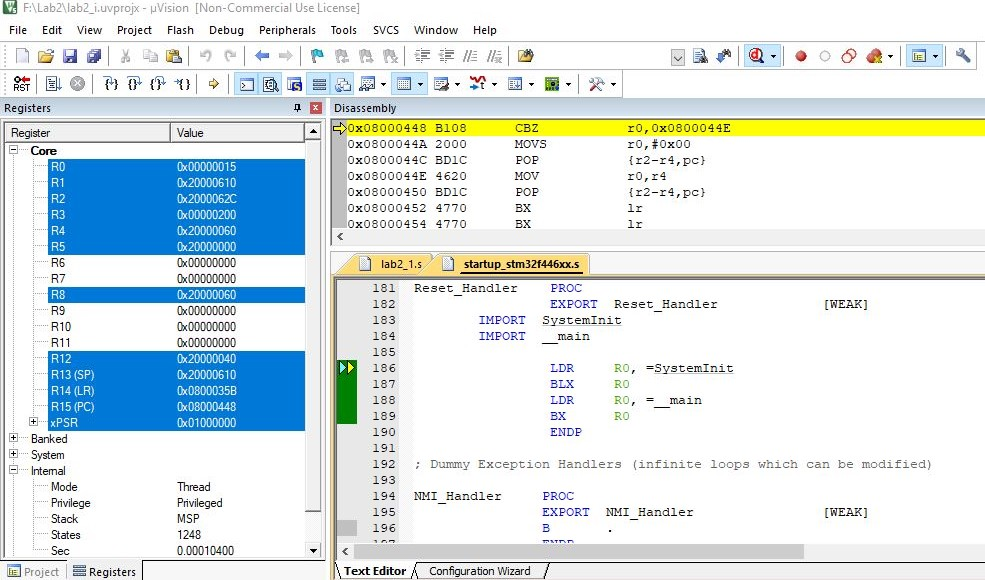
\includegraphics[scale=.7]{images/lab2_ss1.jpg}
    \caption{The system state after loading the code}
    \label{fig:before_task_one}
\end{figure}

\pagebreak

\subsection{Screenshot of the System State after Code Execution:}
\begin{figure}[ht]
    \centering
    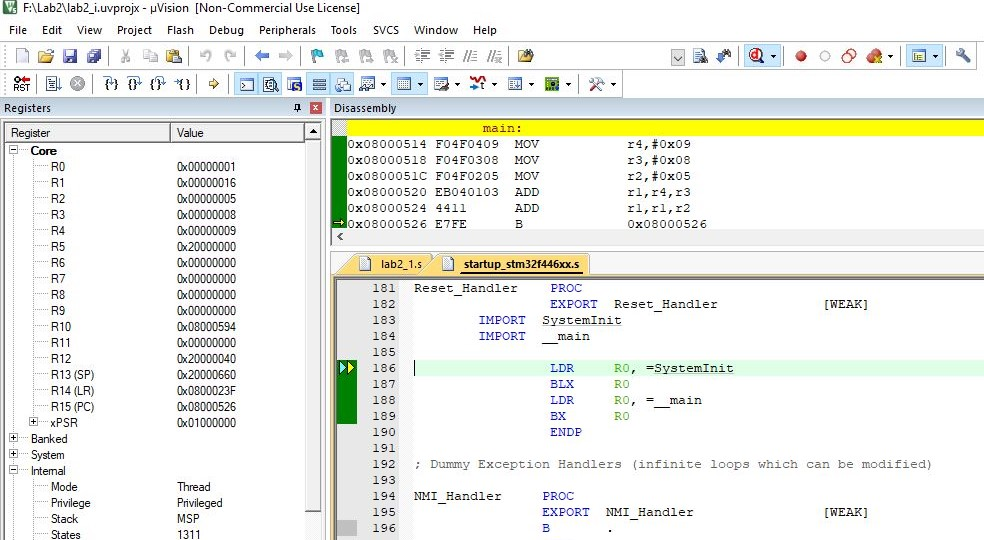
\includegraphics[scale=.7]{images/lab2_ss2.jpg}
    \caption{The system state after executing the code}
    \label{fig:after_task_one}
\end{figure}

\pagebreak

\section{Task 2}

\subsection{Detailed Explanation of the Code:}
The solution to this problem is similar to the previous problem, except that the load register has to be used this time. The solution process is as follows: 
\begin{itemize}
    \item Use the DCD assembler directive to reserve word locations for variables X, Y and Z and initialize them with values 9, 8 and 5 respectively.
    \item Load the registers r4, r3 and r2 with the variables X, Y and Z respectively.
    \item Store the partial sum of X and Y in register r1.
    \item Store the sum of Z and the previously computed partial sum in register r1 and store it in register r0.
\end{itemize}
\subsection{Screenshot of the System State after Loading the Code:}
\begin{figure}[ht]
    \centering
    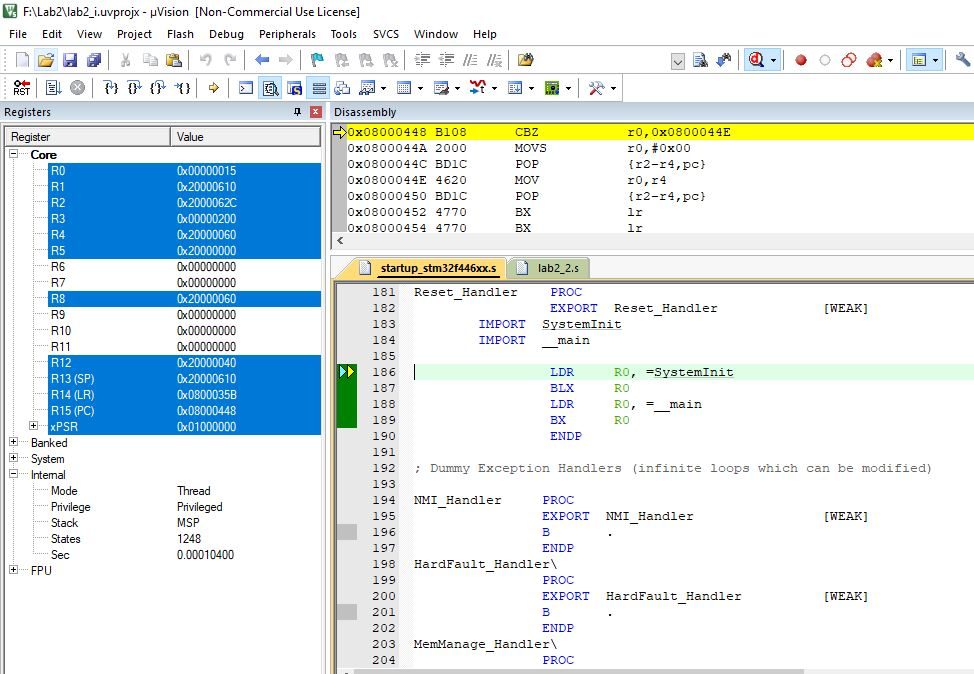
\includegraphics[scale=.7]{images/lab2_ss3.jpg}
    \caption{The system state after loading the code}
    \label{fig:before_task_two}
\end{figure}

\pagebreak

\subsection{Screenshot of the System State after Code Execution:}
\begin{figure}[ht]
    \centering
    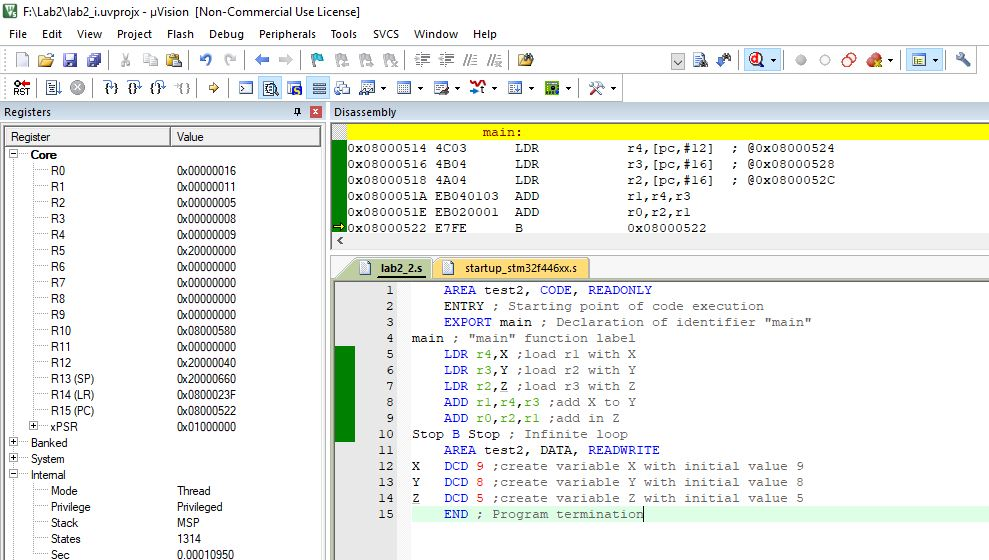
\includegraphics[scale=.7]{images/lab2_ss4.jpg}
    \caption{The system state after executing the code}
    \label{fig:after_task_two}
\end{figure}

\pagebreak

\section{Task 3}

\subsection{Detailed Explanation of the Code:}
This problem asks to perform the addition of two 16-bit variables. The solution process is as follows: 
\begin{itemize}
    \item Store two half-words (16-bit immediate fields) in registers r2 and r3 using MOVW directive.
    \item Store their sum in r1 register sum.
    \item Copy the content of register r1 to r0, to check the rounding in case of overflow.
    \item Use the MOVT directive to load the upper 16-bit field of register r2 with 0's to ensure that the result stays in the range of 16-bit numbers.
    \item Notice that the 17th bit in r1 is 1, but in r0 it is 0.
\end{itemize}
\subsection{Screenshot of the System State after Loading the Code:}
\begin{figure}[ht]
    \centering
    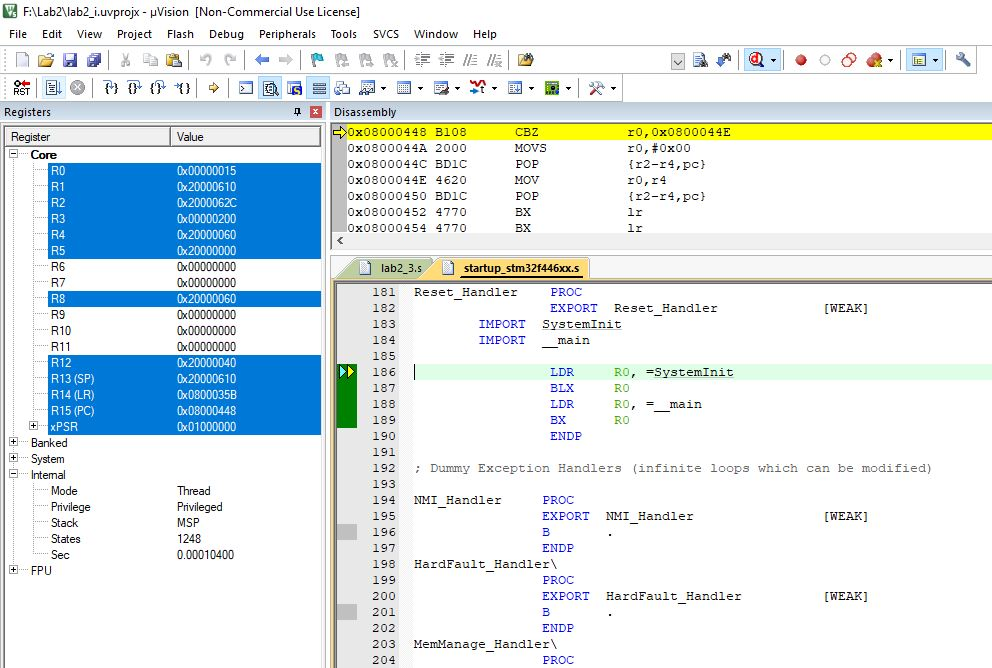
\includegraphics[scale=.7]{images/lab2_ss5.jpg}
    \caption{The system state after loading the code}
    \label{fig:before_task_three}
\end{figure}

\pagebreak

\subsection{Screenshot of the System State after Code Execution:}
\begin{figure}[ht]
    \centering
    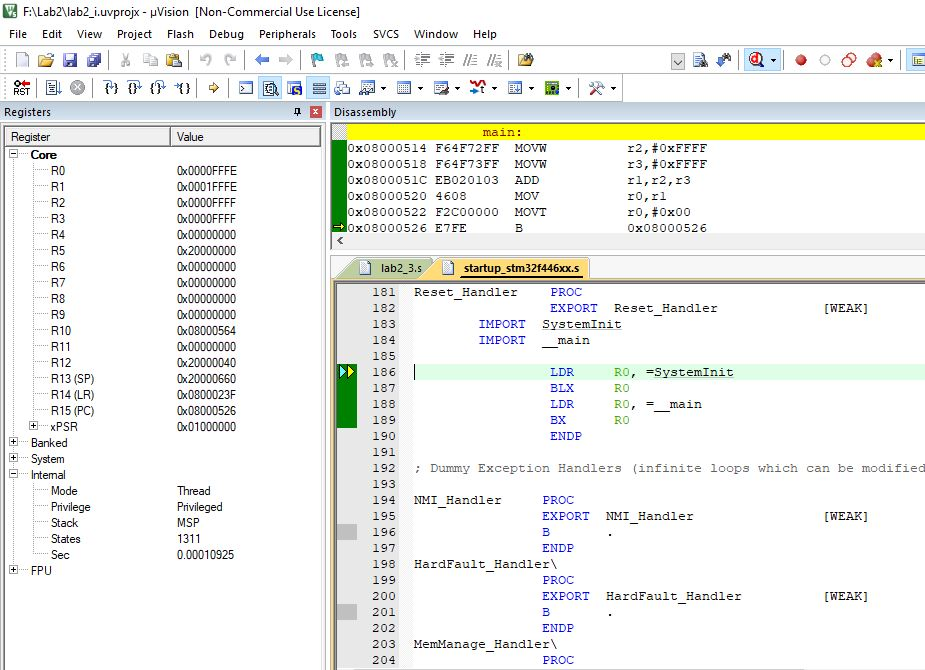
\includegraphics[scale=.7]{images/lab2_ss6.jpg}
    \caption{The system state after executing the code}
    \label{fig:after_task_three}
\end{figure}

\pagebreak


\section{Task 4}

\subsection{Detailed Explanation of the Code:}
This problem asks to find the smaller of two integer numbers. The solution process is as follows: 
\begin{itemize}
    \item Store two arbitrary integers (2 and 3 in this case) in registers r0 and r1.
    \item Use CMP directive to compare the two values.
    \item Use conditional statements MOVLT (less than) and MOVGE (greater than/equal) to find the smaller value and store it in register r2.
\end{itemize}
\subsection{Screenshot of the System State after Loading the Code:}
\begin{figure}[ht]
    \centering
    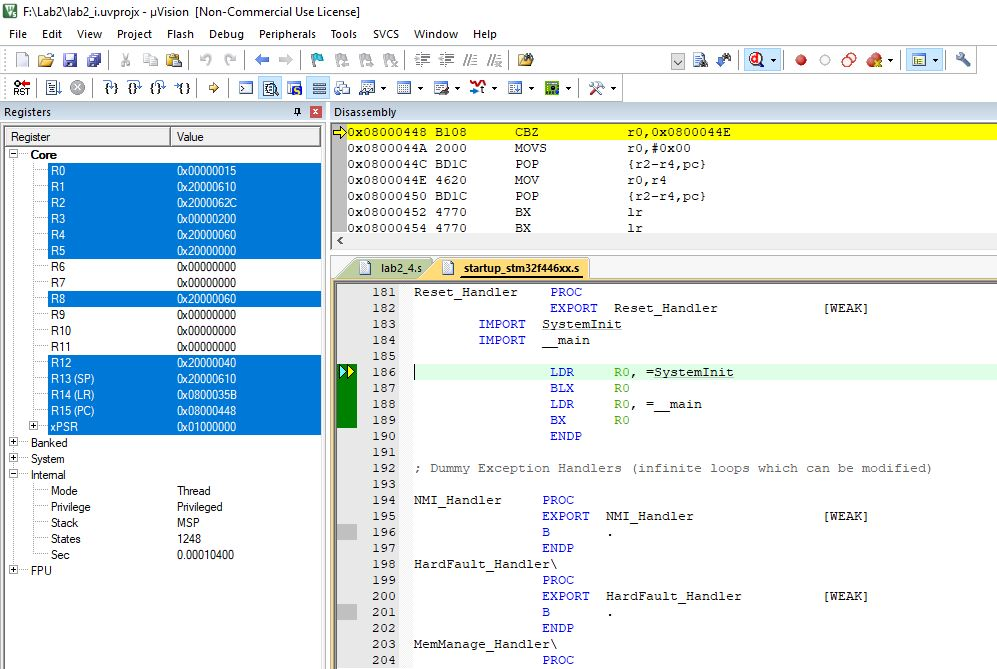
\includegraphics[scale=.7]{images/lab2_ss7.jpg}
    \caption{The system state after loading the code}
    \label{fig:before_task_four}
\end{figure}

\pagebreak

\subsection{Screenshot of the System State after Code Execution:}
\begin{figure}[ht]
    \centering
    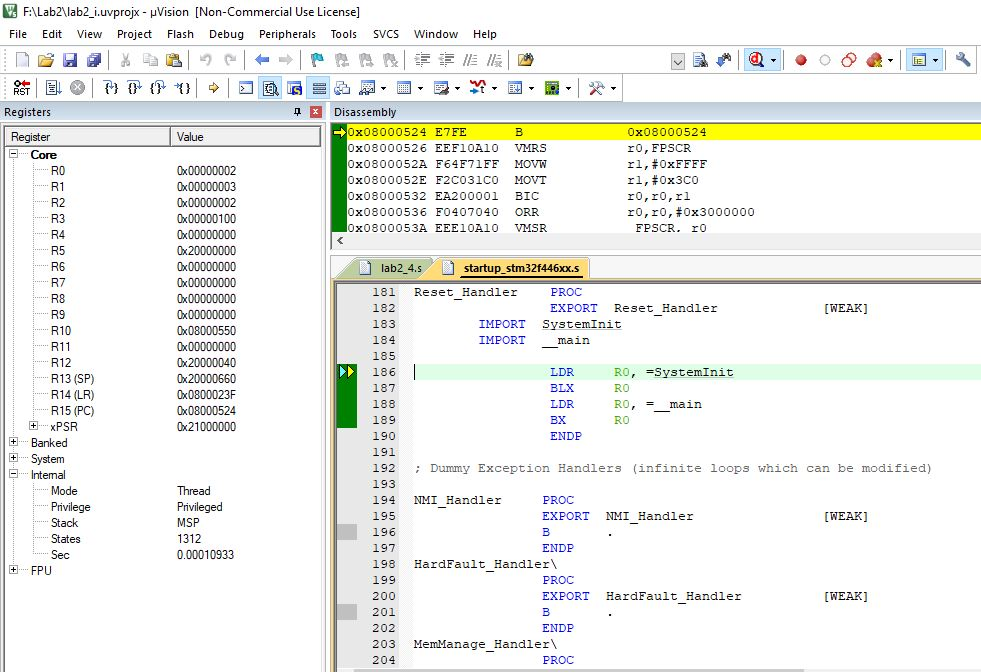
\includegraphics[scale=.7]{images/lab2_ss8.jpg}
    \caption{The system state after executing the code}
    \label{fig:after_task_four}
\end{figure}

\pagebreak



\end{document}
